\documentclass{beamer}
\mode<presentation>
\usepackage{amsmath}
\usepackage{amssymb}
\usepackage{bm}


%\usepackage{advdate}
\usepackage{adjustbox}
\usepackage{subcaption}
%\usepackage{enumitem}
\usepackage{enumerate}
\usepackage{multicol}
\usepackage{mathtools}
\usepackage{listings}
\usepackage{url}
\def\UrlBreaks{\do\/\do-}
\usetheme{Boadilla}
\usecolortheme{lily}
\setbeamertemplate{footline}
{
  \leavevmode%
  \hbox{%
  \begin{beamercolorbox}[wd=\paperwidth,ht=2.25ex,dp=1ex,right]{author in head/foot}%
    \insertframenumber{} / \inserttotalframenumber\hspace*{2ex} 
  \end{beamercolorbox}}%
  \vskip0pt%
}
\setbeamertemplate{navigation symbols}{}

\providecommand{\nCr}[2]{\,^{#1}C_{#2}} % nCr
\providecommand{\nPr}[2]{\,^{#1}P_{#2}} % nPr
\providecommand{\mbf}{\mathbf}
\providecommand{\pr}[1]{\ensuremath{\Pr\left(#1\right)}}
\providecommand{\qfunc}[1]{\ensuremath{Q\left(#1\right)}}
\providecommand{\sbrak}[1]{\ensuremath{{}\left[#1\right]}}
\providecommand{\lsbrak}[1]{\ensuremath{{}\left[#1\right.}}
\providecommand{\rsbrak}[1]{\ensuremath{{}\left.#1\right]}}
\providecommand{\brak}[1]{\ensuremath{\left(#1\right)}}
\providecommand{\lbrak}[1]{\ensuremath{\left(#1\right.}}
\providecommand{\rbrak}[1]{\ensuremath{\left.#1\right)}}
\providecommand{\cbrak}[1]{\ensuremath{\left\{#1\right\}}}
\providecommand{\lcbrak}[1]{\ensuremath{\left\{#1\right.}}
\providecommand{\rcbrak}[1]{\ensuremath{\left.#1\right\}}}
\providecommand{\rank}{\text{rank}}
\theoremstyle{remark}
\newtheorem{rem}{Remark}
\newcommand{\sgn}{\mathop{\mathrm{sgn}}}
\providecommand{\abs}[1]{\left\vert#1\right\vert}
\providecommand{\res}[1]{\Res\displaylimits_{#1}} 
\providecommand{\norm}[1]{\lVert#1\rVert}
\providecommand{\mtx}[1]{\mathbf{#1}}
\providecommand{\mean}[1]{E\left[ #1 \right]}
\providecommand{\fourier}{\overset{\mathcal{F}}{ \rightleftharpoons}}
%\providecommand{\hilbert}{\overset{\mathcal{H}}{ \rightleftharpoons}}
\providecommand{\system}{\overset{\mathcal{H}}{ \longleftrightarrow}}
	%\newcommand{\solution}[2]{\vec{Solution:}{#1}}
%\newcommand{\solution}{\noindent \vec{Solution: }}
\providecommand{\dec}[2]{\ensuremath{\overset{#1}{\underset{#2}{\gtrless}}}}
\newcommand{\myvec}[1]{\ensuremath{\begin{pmatrix}#1\end{pmatrix}}}
\newenvironment{amatrix}[1]{%
  \left(\begin{array}{@{}*{#1}{c}|c@{}}
}{%
  \end{array}\right)
}
\let\vec\mathbf

\lstset{
%language=C,
frame=single, 
breaklines=true,
columns=fullflexible
}

%\numberwithin{equation}{section}

\title{Matgeo-4.13.4}
\author{Harichandana Varanasi-ai25btech11039}

\date{\today} 
\begin{document}

\begin{frame}
\titlepage
\end{frame}

\section*{Outline}

\begin{frame}
\frametitle{Question}

\noindent\textbf{Q-4.13.4} \;
$y=10^{x}$ is the reflection of $y=\log_{10}x$ in the line whose equation is \underline{\hspace{3cm}}.

\end{frame}
\begin{frame}{Solution}
    \renewcommand{\theequation}{\arabic{equation}}

Let the mirror line be written in normal form
\begin{equation}
  \vec{n}^{\top}\vec{x}=c,                                   \label{eqL}
\end{equation}
with normal $\vec{n}\in\mathbb{R}^{2}$ and variable vector $\vec{x}\in\mathbb{R}^{2}$.


A point on the curve $y=\log_{10}u$ is
\begin{equation}
    \vec{Q}(t)=\myvec{t\\ \log_{10}t}, \qquad t>0 .
\end{equation}


Its reflection in the line \eqref{eqL} is 
\begin{equation}
  \vec{R}(t)=\vec{Q}(t)-\frac{2\big(\vec{n}^{\top}\vec{Q}(t)-c\big)}{\|\vec{n}\|^{2}}\;\vec{n}. \label{eqR}
\end{equation}
For the image curve to be  $y=10^{x}$ we require
\begin{equation}
  \vec{R}(t)=\myvec{\log_{10}t\\ t}\quad \text{for all } t>0 . \label{eqTarget}
\end{equation}

Equating components in \eqref{eqR}--\eqref{eqTarget} and collecting the
independent functions $t$ and $\log_{10}t$ yields
\end{frame}
\begin{frame}{Solution}
    \begin{equation}
  a^{2}=b^{2}, \qquad a\,b=-a\,b, \qquad c=0 .
\end{equation}
Hence $a=-b\neq 0$ and $c=0$.  Thus $\vec{n}\propto\myvec{1\\ -1}$ and the mirror line is
\begin{equation}
  \myvec{1 & -1}\vec{x}=0.                                   \label{eqAns}
\end{equation}

Therefore, the required line of reflection is
\[
  \boxed{\ \myvec{1\;\; -1}\vec{x}=0\ }\quad (\text{scalar form } y=x).
\]
\endgroup
\end{frame}


\begin{frame}{Plot}
    \begin{figure}[H]
    \centering
    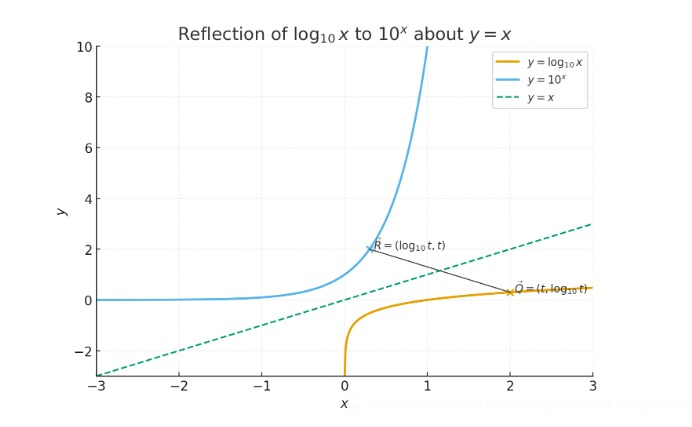
\includegraphics[width=0.8\linewidth]{figs/matgeo-4.13.4.jpeg}
    \caption{$y=\log_{10}x$ and $y=10^{x}$ with mirror line $y=x$.}
    \label{fig:4.13.4}
\end{figure}
\end{frame}

\end{document}
